\chapter{Aplicación}

    \section{Función de la aplicación}
        La aplicación móvil tiene como objetivo mostrarle al usuario los distintos tipos de valores de la batería en tiempo real. Esto lo hará por medio de pantallas destinadas a los valores e interacciones que necesite el usuario, contando con gráficos interactivos. Los datos mostrados en la aplicación son subidos desde una base de datos. Contando también con una sección para contactarnos, por medio de nuestras redes sociales y página web.\par
        Con esta aplicación, el usuario podrá saber, en todo momento, los valores que necesite de la batería, como por ejemplo, la entrega que tiene la batería hacia el dispositivo que esté alimentando o, para un perfil más técnico, valores del panel solar y gráficos para más detalles sobre la misma.\par

    \section{Desarrollo del mockup de la aplicación}
    
        \subsection{Mockup}
            	Para poder desarrollar la aplicación, se necesita tener un Mockup. Su función es proveer al desarrollador el prototipo de funcionamiento, planteado de forma ilustrativa, el cual, da un primer vistazo estético, funcional e informativo de cómo será la misma. \par
                Esto conlleva plantear el diseño, e información que contendrá la aplicación , para que, posteriormente, el desarrollo final de la aplicación, se base en el Mockup, siendo de esta forma, más cómodo y práctico poder desarrollarla.\par
                La página que se designó para realizar el Mockup, fue “\href{https://marvelapp.com}{Marvel}”.\par
                Dentro de este, pueden haber varios cambios según vaya avanzando y se necesite, ya que, al fin y al cabo, es a modo ilustrativo para después poder desarrollar la aplicación final.\par
                
                \begin{figure}[H]
                    \centering
                    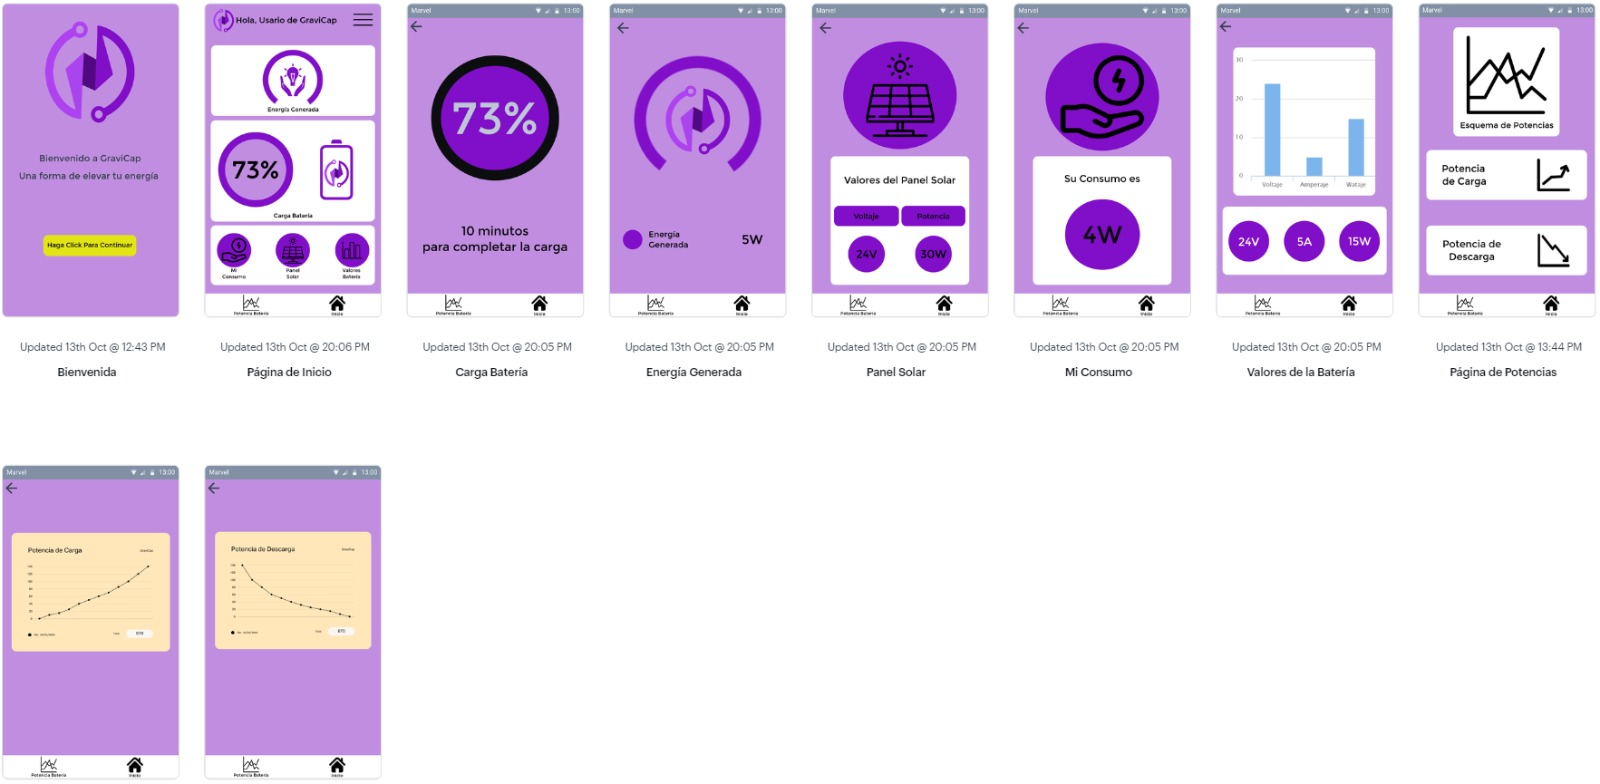
\includegraphics[width=0.8\linewidth]{Aplicación/Mockup.png}
                    \caption{Mockup de la aplicación.}
                    \label{fig:a14}
                \end{figure}
                
            \subsection{UI/UX}
                La \textbf{UX} (Experiencia de Usuario) es la experiencia integral y el conjunto de interacciones que tienen los usuarios con la misma.\par
                En cuanto a la \textbf{UI} (Interfaz de Usuario) consiste en toda la arquitectura de información, patrones y diferentes elementos visuales que nos permitan explorar la funcionalidad de la aplicación de forma eficaz y gratificante.\par
                Con esto, el usuario podrá tener una interacción “amigable” con la aplicación, siendo más cómodo y práctico moverse dentro de la misma para ver lo que necesite.\par
                La diferencia entre estos, es que la UX se centra en la manera en que el usuario interactúa con el producto de manera eficaz y, por otro lado, la UI busca ofrecer una experiencia estética satisfactoria.\par

            \subsection{User Journey}
                Para el desarrollo de la aplicación se planteó utilizar como metodología, una “jornada de usuario”. Esta metodología, plantea un mapa de recorrido del usuario en nuestra aplicación, representando así, su experiencia visual e interactiva con la misma. Pudiendo así, plantear el desarrollo del Mockup enfocándonos en el proceso que realizaría nuestro usuario dentro de la aplicación y su perspectiva.\par
                El proceso para esta metodología es buscar la empatía con el usuario, comprendiendo la relación y puntos de contacto que este tiene. Analizar sus acciones y procesos, para así, determinar lo que necesita. Con esto, se puede generar una mejor experiencia para el usuario y un proceso más eficiente.\par
                Facilita tanto el desarrollo de la aplicación como el proyecto en sí, generando una experiencia del usuario y requerimientos para el mismo. También se relaciona directamente con la UI/UX y facilita un mejor y cómodo planteamiento para las mismas.\par
                Esta herramienta o metodología, nos permite generar un usuario para así comprender y mejorar su experiencia dentro de la aplicación, así también, dándonos un mejor desarrollo dentro de nuestro proyecto.\par

                
        \section{Estructura de la Aplicación}
        
            \subsection{Editor de Código y Framework}
                Para el desarrollo de la aplicación, se utilizó el editor de código “Visual Studio Code”, en conjunto con “\href{https://ionicframework.com}{Ionic}" un framework de código abierto, proporcionandonos comodidad y amplias opciones de herramientas para el desarrollo, conteniendo varias opciones para la implementación en varios lenguajes.
                
            \subsection{Lenguajes Utilizados}
                Los lenguajes utilizados fueron HTML, CSS, JS y, como principal, React. Siendo este último, el lenguaje principal para el uso de las herramientas que nos provee Ionic.\par
                
        \section{Componentes}
        
            \subsection{WelcomePage.tsx}
            
                Este componente es el primero que se ve al iniciar la aplicación, su función consta de darle una pequeña bienvenida al usuario, explicando un poco sobre la batería y el proyecto, con un botón que lo envía a la pantalla de inicio una vez que el usuario quiera.\par

                \begin{figure} [H]
                    \centering
                    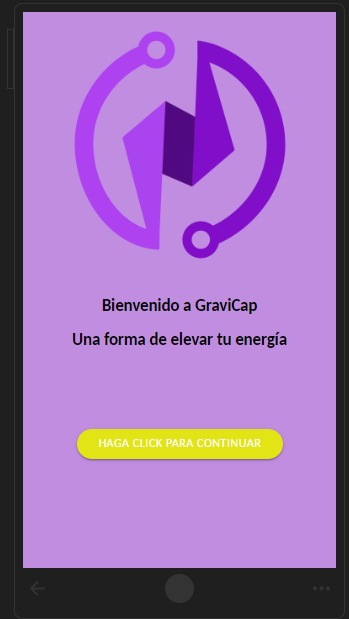
\includegraphics[width=0.25\linewidth]{Aplicación/Welcome.png}
                    \caption{Página de Bienvenida}
                    \label{fig:a1}
                \end{figure}
                
            \subsection{StartPage.tsx}
                Una vez vista la pantalla de bienvenida, el usuario es reenviado hacia la pantalla de inicio, la cual, es la pantalla principal de la aplicación, esta contiene los botones con links hacia las distintas pantallas de valores. También consta de los tabs, los cuales nos van a permitir movilizar al usuario hacia la página de los gráficos de potencia.\par
                En el apartado de arriba a la derecha encontramos un botón de información, el cual contiene los links hacia nuestro contacto y diversas redes sociales.\par

                \begin{figure} [H]
                    \centering
                    \begin{subfigure}{0.4\textwidth}
                        \centering
                        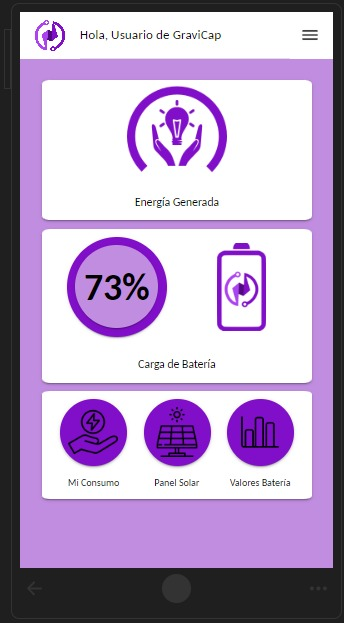
\includegraphics[width=0.7\textwidth]{Aplicación/Start.png}
                        \caption{Página de Inicio}
                        \label{fig:a2.1}
                    \end{subfigure}
                    \begin{subfigure}{0.4\textwidth}
                        \centering
                        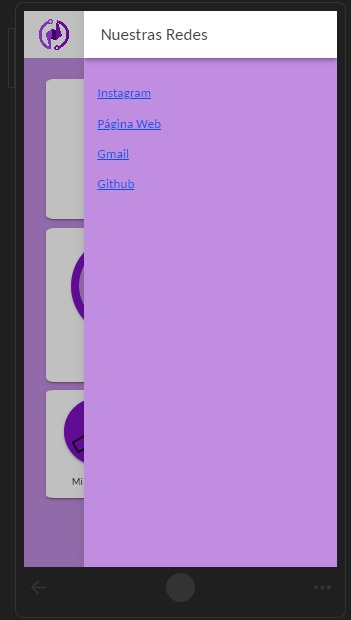
\includegraphics[width=0.7\textwidth]{Aplicación/Start_Menu.png}
                        \caption{Menú de Inicio}
                        \label{fig:a2.2}
                    \end{subfigure}
                    \hfill
                            
                    \caption{Ambas partes de la Página de Inicio}
                    \label{fig:a2}
                    \end{figure}
                
            \subsection{GeneratedEnergy.tsx}
                Este componente contiene un valor importante y recurrente para el usuario, el cual es la energía generada por la batería. Este valor le provee al usuario el valor de cuánta potencia está entregando hacia su dispositivo.\par

                \begin{figure} [H]
                    \centering
                    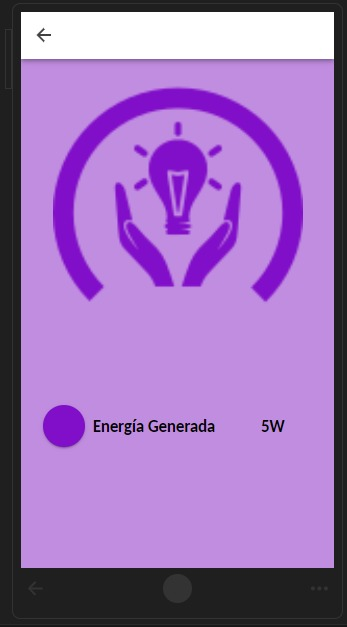
\includegraphics[width=0.25\linewidth]{Aplicación/Generated.png}
                    \caption{La cantidad de energía generada (Los valores son de referencia)}
                    \label{fig:a3}
                \end{figure}
                
            \subsection{BatteryCharge.tsx}
                Para el usuario, también es importante saber cuál es la carga de la batería, es decir, en este caso, si está en su punto más alto o más bajo. Este valor se basa en un porcentaje, el cual nos indica la posición del peso de la batería, que se traduce en un valor porcentual para el usuario. Por ejemplo, el 100\% de la batería, se da cuando el peso está en su punto más bajo, ya habiendo transformado toda la energía potencial.\par

                \begin{figure} [H]
                    \centering
                    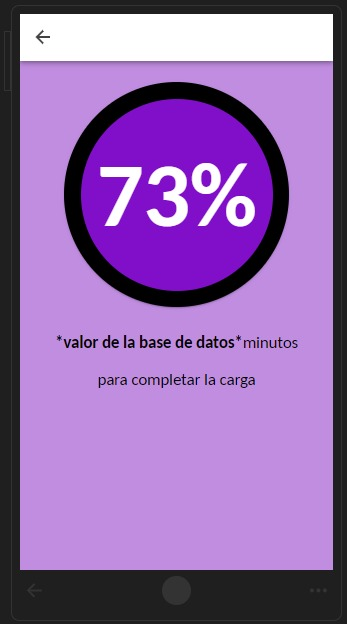
\includegraphics[width=0.25\linewidth]{Aplicación/Charge.png}
                    \caption{Carga de la batería (Los valores son de referencia)}
                    \label{fig:a4}
                \end{figure}
                
            \subsection{MyConsumption.tsx}
                El usuario también necesita saber el consumo de su dispositivo. Ese es el funcionamiento de este componente. Dándole el valor en unidad de potencia.\par

                \begin{figure} [H]
                    \centering
                    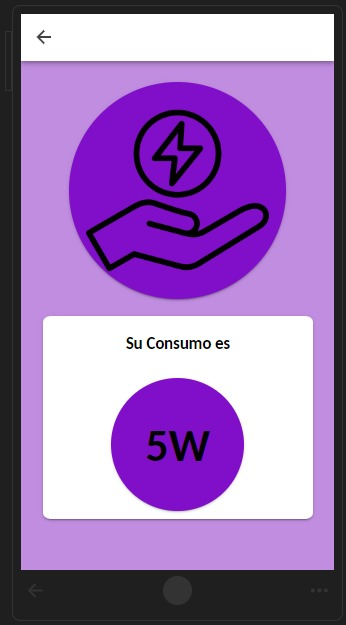
\includegraphics[width=0.25\linewidth]{Aplicación/Consumption.png}
                    \caption{El consumo del usuario (Los valores son de referencia)}
                    \label{fig:a5}
                \end{figure}
                
            \subsection{SolarPanel.tsx}
                Para saber los valores de entrega del panel solar, el usuario puede verlos dentro de la pantalla del panel solar.\par
                Los valores que nos da son el voltaje que entrega y su potencia. Todo esto en tiempo real.\par

                \begin{figure} [H]
                    \centering
                    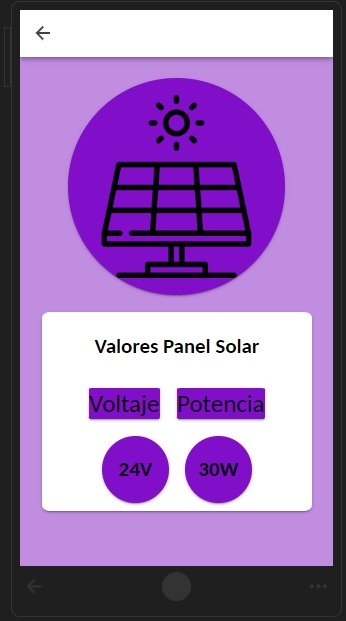
\includegraphics[width=0.25\linewidth]{Aplicación/Value_Energy.png}
                    \caption{Valor del panel solar utilizado (Los valores son de referencia)}
                    \label{fig:a6}
                \end{figure}
                
            \subsection{BatteryValues.tsx}
                Para registrar la batería y sus valores varios, en la pantalla de valores de batería el usuario podrá ver valores como Voltaje, Corriente y Potencia de la batería.\par

                \begin{figure} [H]
                    \centering
                    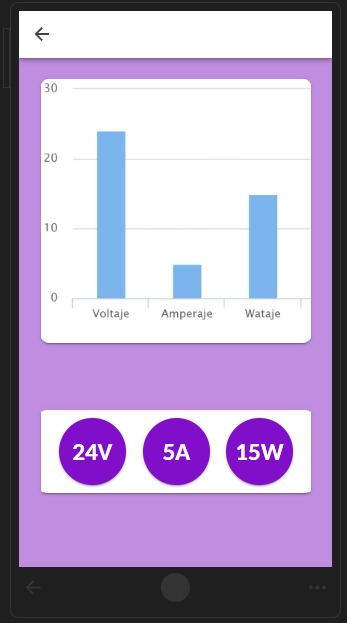
\includegraphics[width=0.25\linewidth]{Aplicación/Value_Battery.png}
                    \caption{Valor de la batería (Los valores son de referencia)}
                    \label{fig:a7}
                \end{figure}

            \subsection{GraphicsPage.tsx}
                En este apartado, el cual el usuario puede acceder desde el tab, encontraremos dos botones los cuales contienen los gráficos de carga y descarga de la batería.\par

                \begin{figure} [H]
                    \centering
                    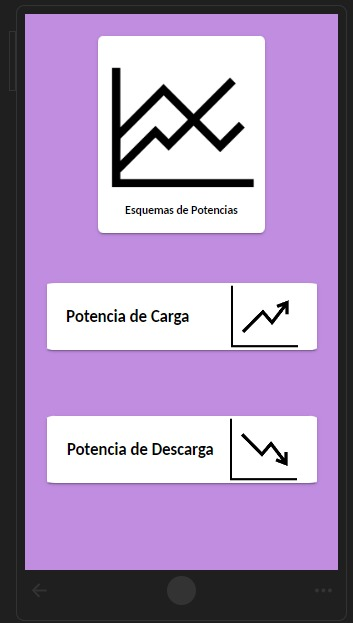
\includegraphics[width=0.25\linewidth]{Aplicación/Graphics_Page.png}
                    \caption{Página de Gráficos}
                    \label{fig:a8}
                \end{figure}

            \subsection{ChargingPowerGraphics.tsx}
                En este encontramos un gráfico de carga, el cual se basa en la potencia que entrega la batería en función del tiempo.\par
                Este funciona cuando la batería se encuentra en estado de carga, es decir, cuando está ascendiendo. Será un gráfico en ascenso.\par

                \begin{figure} [H]
                    \centering
                    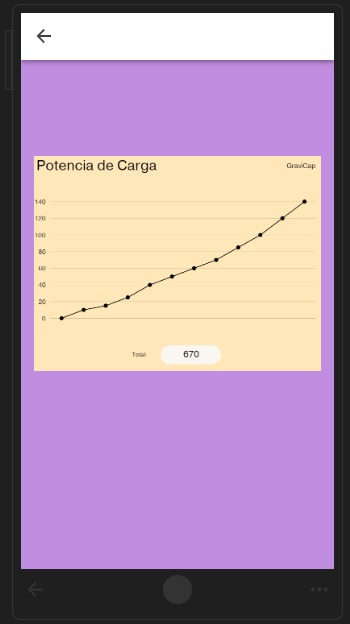
\includegraphics[width=0.25\linewidth]{Aplicación/Graphics_Charge.png}
                    \caption{Gráfico de Carga (Los valores son de referencia)}
                    \label{fig:a9}
                \end{figure}

            \subsection{DischargePowerGraphics.tsx}
                En este encontramos un gráfico de descarga, el cual se basa en la potencia que entrega la batería en función del tiempo.\par
                Este funciona cuando la batería se encuentra en estado de descarga, es decir, cuando está descendiendo. Será un gráfico en descenso.\par

                \begin{figure} [H]
                    \centering
                    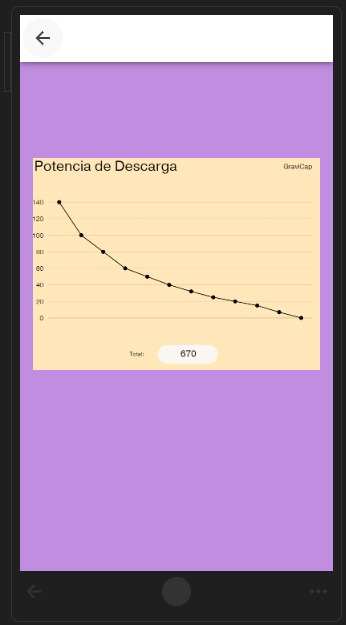
\includegraphics[width=0.25\linewidth]{Aplicación/Graphics_Discharge.png}
                    \caption{Gráfico de Descarga (Los valores son de referencia)}
                    \label{fig:a10}
                \end{figure}

            \subsection{Tabs.tsx}
                Este componente es la barra de botones que se encuentra en la parte de abajo, este contiene un botón que te redirecciona hacia la pantalla de inicio y otra que te redirecciona hacia la parte los gráficos de potencia. Dándole una mayor accesibilidad al usuario hacia las pantallas del Tab.\par

            \subsection{main.tsx}
                El main es un componente el cual no es visible, dentro de la aplicación. Este se encarga de poder ejecutar las rutas declaradas dentro del archivo App.tsx.\par

            \subsection{App.tsx}
                Este componente tampoco es visible, ya que se encarga de declarar las rutas dentro de la aplicación. Por ejemplo, puede realizar que al abrir la aplicación, redireccione al usuario hacia la pantalla de bienvenida.\par
                
        \section{Desarrollo}
            Para el desarrollo de la aplicación, se descargó \textbf{Ionic}, configurando su descarga para la utilización de herramientas y templates con el lenguaje de programación de \textbf{React}. Para poder programar y utilizar las herramientas descargadas se utilizó el editor de código de \textbf{Visual Studio Code}.\par 
            \subsection{Base de Datos}
                Teniendo como base de desarrollo el Mockup, facilita la programación de la misma. También cabe resaltar que mediante se desarrolla la aplicación en sí, el Mockup puede ir variando o la aplicación puede no ser completamente fiel estética y visualmente al mismo, quedando la aplicación final, diferente al Mockup, esto ya que se utiliza como una primera base.\par 
                Mediante el proceso se encuentran nuevas herramientas que se adapten mejor a las necesidades del momento, reescribiendo o modificando el Mockup según se requiera para una mejor versión de la aplicación.\par
            \subsection{Creación de Archivos}
                Se crearon los distintos archivos que funcionarán como componentes para la creación de las pantallas de la aplicación, desarrollando y programando así la estructura de cada uno, importando las carpetas y herramientas para cada archivo.\par

            \subsection{Herramientas de Ionic}
                Para el desarrollo de programación de los archivos se necesitó tener conocimientos dentro del lenguaje de HTML para poder programar su estructura y combinarse con el lenguaje principal React y las herramientas que provee, creando así, componentes .tsx como archivos principales para el desarrollo. En cuanto a las herramientas que nos provee Ionic, se investigó en el Framework sobre sus templates e información del uso de las herramientas más convenientes para el desarrollo de los archivos. Para poder estilizarlos según queramos, se necesitó también tener conocimientos en CSS. Para los gráficos, importados de carpetas, se necesitó tener conocimientos básicos en JavaScript.\par
                    \subsubsection{Herramientas Principales Utilizadas en Ionic}
                        Para el desarrollo de la aplicación, se utilizaron varias herramientas que nos provee Ionic, pero algunas son de características más importantes e importante resaltar, ya sea porque se utilizaron varias veces en muchos archivos, o por el peso que tienen dentro del desarrollo.\par
                        \subsubsubsection{IonApp}
                            Para la creación de los archivos, se necesita empezar con una constante o función, en la cual iremos desarrollando el código para la creación de las pantallas, así como declarar primeramente una herramienta IonApp la cual contendrá el código y los elementos de la aplicación de Ionic, solamente se declara uno en el archivo que queramos considerar como principal.\par
                        \subsubsubsection{IonContent}
                            Otro componente importante para el desarrollo es declarar un IonContent el cual actúa de contenedor principal de los componentes de la aplicación, dando así, un área única para el contenido por fuera del Header.\par
                        \subsubsubsection{IonHeader y IonMenu}
                            IonHeader componente que actúa de barra superior central, conteniendo componentes tales como iconos, botones y texto (vistos en el Header de la pantalla de Inicio). En este mismo también se declara el componente IonMenu, un botón de información lateral ubicado en la parte superior derecha de la pantalla de inicio, proporcionando los links hacia nuestras redes sociales, contacto y página web.\par
                        \subsubsubsection{IonCard}
                            Un componente muy utilizado es el de IonCard visto en gran parte en la pantalla de inicio y utilizado en otros archivos. Actuando de contenedor de otros componentes y, a su vez, dándole una mejor estética, actuando, como dice su nombre, como una carta. Modificándose en cuanto a estilos y formas con CSS, pueden actuar de contenedores circulares, también vistos en los contenedores de "Mi Consumo", "Panel Solar" y "Valores de Batería" en la pantalla de inicio. También dándole un recuadro en las páginas de gráficos, y actuando como "botones" (declarados con el componente de NavLink los cuales, al clickearlos, nos redireccionan hacia otra pantalla.\par
                        \subsubsubsection{IonNavLink y IonBackButton}
                            Con los archivos desarrollados con sus componentes y estructuras, para el movimiento del usuario por las diferentes pantallas de estas, estos necesitan un enrutamiento para la conexión entre sí. Para esto, los componentes que provee Ionic como botones (ion-button) o cartas (ion-card) se los programó con la función de IonNavLink, funciona como un enrutamiento, el cual realiza que al clickear un botón o carta nos redireccione hacia otro componente/archivo que le designemos. Con esto, el Usuario se puede movilizar dentro de la aplicación hacia donde necesite. Así también como se redirecciona hacia un componente, puede volver hacia atrás a la pantalla anterior, esto con la herramienta IonBackButton.\par
                        \subsubsubsection{IonButton}
                            Para una mejor interacción y movimiento del usuario dentro de la aplicación, se implementaron botones (ion-button). Por ejemplo, en la pantalla de Bienvenida. Otros ubicados en la parte inferior de la página de Inicio y de Gráficos la cual le permite al usuario moverse de una forma más eficiente entre las mismas. Estos cumplen la función de redireccionar al usuario hacia su determinada pantalla, dándole posibilidad de visualizar otras pantallas y obtener otro tipo de información.\par
                        \subsubsubsection{Formato SmartPhone}
                            Ionic también nos provee una herramienta para poder ver el desarrollo del archivo que estemos programando dentro de Visual Studio Code en forma de un SmartPhone. Con esta función se facilita poder programar cada componente estructural para el desarrollo final.\par
                            
                            \begin{figure}[H]
                                \centering
                                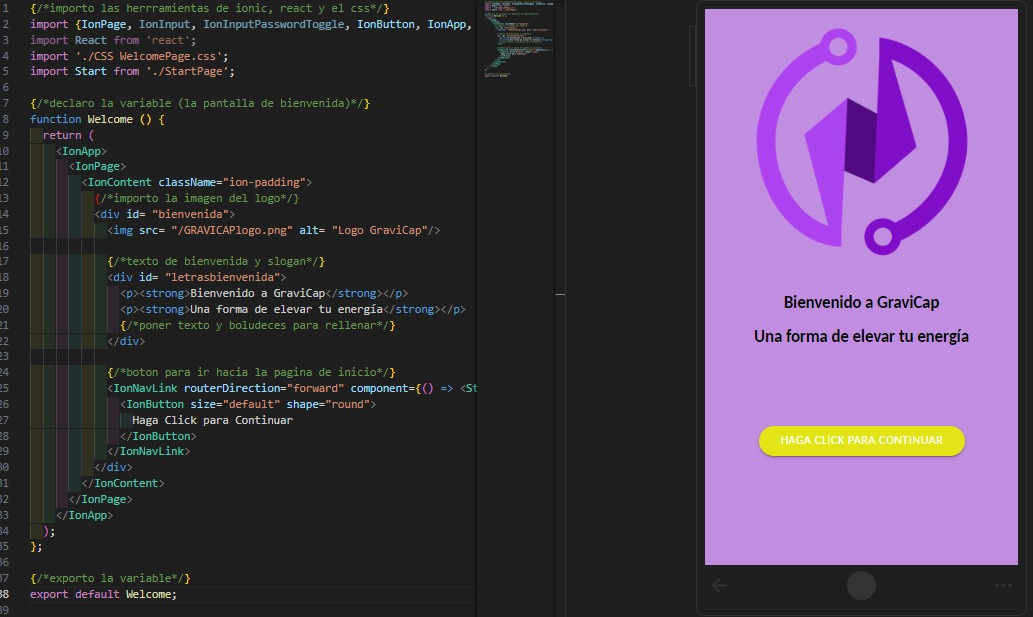
\includegraphics[width=\linewidth]{Aplicación/Code.png}
                                \caption{Imagen de Referencia de la función de Smartphone}
                                \label{fig:a15}
                            \end{figure}
                
                            Con los archivos desarrollados con sus componentes y estructuras, para el movimiento del usuario por las diferentes pantallas de estas, los componentes necesitan un enrutamiento para la conexión entre sí. Para esto, los componentes que provee Ionic como botones (\textit{ion-button}) o cartas (\textit{ion-card}) se los programó con la función de \textit{IonNavLink}, funciona como un enrutamiento, el cual realiza que al clickear un botón o carta nos redireccione hacia otro componente/archivo que le designemos. Con esto, el Usuario se puede movilizar dentro de la aplicación hacia donde necesite. Así también como se redirecciona hacia un componente, puede volver hacia atrás a la pantalla anterior, esto con la herramienta \textit{IonBackButton}.\par
                El usuario, en la pantalla de inicio, en la parte superior derecha de la misma, dispone de un botón de información, el cual, le proveerá información de nuestras redes sociales y contacto.\par
                Para un mejor movimiento del usuario dentro de la aplicación, se implementó la herramienta \textit{Tabs} (\textit{ion-tabs}). Esta es una barra ubicada en la parte inferior la cual le permite al usuario moverse de una forma más eficiente, conteniendo iconos, los cuales actúan de botones para redireccionar al usuario hacia su determinada pantalla, dándole posibilidad de visualizar otras pantallas y obtener otro tipo de información.\par
                Una vez teniendo todos los archivos programados con sus respectivas estructuras y componentes, se debe añadir estilos, darle forma a los componentes que queramos, colores y tamaños, dándoles así el vistazo estético requerido planteado en el Mockup. Para esto, cada componente necesita sus estilos, creándose así un archivo \textit{CSS} individual para cada uno. Estos se programan y se importan al archivo que se requiera, modificando su estructura y tamaños dándole un mejor acabado estético para el usuario.\par
            \subsection{Estilos y CSS}
                Una vez teniendo todos los archivos programados con sus respectivas estructuras y componentes, se debe añadir estilos, darle forma a los componentes que queramos, colores y tamaños, dándoles así el vistazo estético requerido planteado en el Mockup. Para esto, cada componente necesita sus estilos, creándose así un archivo CSS individual para cada uno. Estos se programan y se importan al archivo que se requiera, modificando su estructura y tamaños dándole un mejor acabado estético para el usuario.\par
            \subsection{Gráficos}
            \subsection{Servidor}